\chapter{Activity}
Activity는 앱에서 화면의 기본단위이고 setContentView() 메서드로 메인 뷰를 화면에 표시한다.
때에 따라 setContentView()를 실행하지 않고, 로직 분기를 해서 다른 Activity를 띄우는 용도로 사용하기도 한다.
한 예로 Intent의 스킴(scheme)에 따라 여러 화면을 호출하는 경우가 있다. 
이때 AndroidManifest.xml에서 여러 Activity에 intent-filter 엘리먼트를 추가하지 않고, Controller 역할의 Activity 1개에만 여러 스킴의 intent-filter를 명시해서 Controller Activity를 거쳐 다른 화면으로 이동시킨다.\\

Activity는 AndroidManifest.xml에 선언해야 호출 가능하다. 
Activity를 설정 파일에 추가할 뿐이지만, 개수가 많으면 유지에 어려움이 있으므로\footnote{규모가 있는 앱은 기능이 변경되면서 쓰지 않는 Activity가 자꾸 생겨나기도 한다. 다행히 근래의 IDE에서는 쓰지 않는 Activity를 표시해주기도 한다.}, Activity는 불필요하게 많이 만들지 않는 것을 권장한다.
내부에 UI 액션이 많고 로직이 많다면 우선 Activity를 고려하고, 
다른 Activity 위에 팝업 형식으로 뜬다면 커스텀 레이아웃 다이얼로그나 DialogFragment, PopupWindow로 대체를 고려하자.
`로딩중'이라고 전체를 덮는 반투명 화면은 어떨까? 이것도 Activity보다는 DialogFragment가 적절하다.
기준은 단순하게 하자. 독립적인 화면이라고 하면 Activity가 더 적합하고, 종속적인 화면으로 보이면 다른 것을 쓸 수 있는지 생각해보자.\\

\section{생명주기}
%http://developer.android.com/training/basics/activity-lifecycle/pausing.html
Activity의 생명주기를 정확히 이해하는 것은 중요하다. 
생명주기를 이해하지 못했을 때 리소스가 반납되지 않을 수도 있고, 필요한 데이터를 읽어들이지 못할 수도 있다.

% http://developer.android.com/guide/topics/fundamentals/activities.html 기본 참고
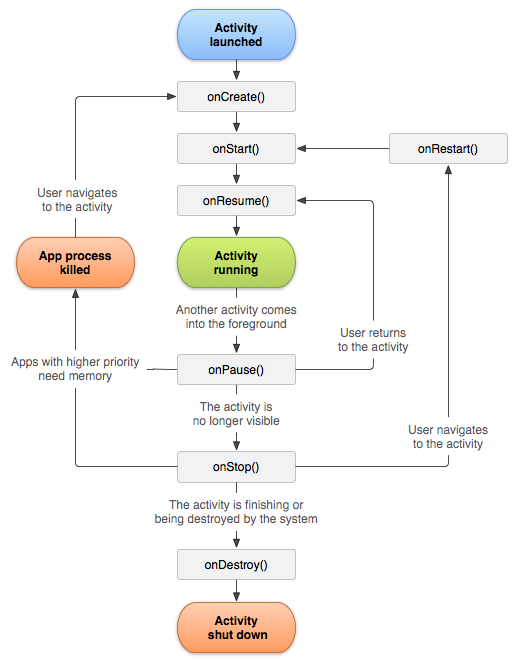
\includegraphics[scale=0.5]{activity-lifecycle}

onStop(), onDestroy() 메서드는 반드시 실행된다는 보장이 없다. 일반적으로 onCreate(), onResume(), onPause() 메서드를 오버라이드하고, 리소스를 안전하게 정리하는 데 필요하다면 onStop()이나 onDestroy()에 안전장치로 코드를 추가하는 경우가 있다.\\

케이스별로 생명주기 메서드가 호출되는 순서를 알아보자.\label{flow}

\fbox{\bfseries 시작할 때}
onCreate $\rightarrow$ onStart $\rightarrow$ onResume\\

\fbox{\bfseries 화면 회전할 때(가로/세로)}
onPause $\rightarrow$ onStop $\rightarrow$ onDestroy $\rightarrow$ onCreate $\rightarrow$ onStart $\rightarrow$ onResume\\

\fbox{\bfseries 다른 Activity가 위에 뜰 때/Power 키로 화면 OFF할 때/Home 키}
onPause $\rightarrow$ onStop\\

\fbox{\bfseries Back 키로 Activity 종료}
onPause $\rightarrow$ onStop $\rightarrow$ onDestroy\\

\fbox{\bfseries Back 키로 기존 Activity에 돌아올 때/Home 키로 나갔다가 돌아올 때}
onRestart $\rightarrow$ onStart $\rightarrow$ onResume\\

\fbox{\bfseries 다이얼로그 테마 Activity가 위에 뜰 때/투명 Activity가 위에 뜰 때}
onPause
\\

메서드가 어디까지 호출되는 지는 visible 상태와 포그라운드 상태를 체크해보면 좀 더 알기 쉽다.
onPause()까지 실행하면 백그라운드이면서 visible 상태이고 onStop()까지 실행되면 not visible 상태이다. 
Activity API 문서에 보면 세 가지 lifetime으로 구분한 내용이 있다.
\begin{itemize}
\item entire lifetime: onCreate() $\sim$
 onDestroy()
\item visible lifetime: onStart() $\sim$
 onStop()
\item foreground lifetime: onResume() $\sim$
 onPause()
\end{itemize}
여기서 혼동되는 게 있다. onCreate() 메서드 내에서 setContentView()에 넣은 레이아웃이 onStart()에서부터 화면에 보이는 것일까? 그렇지 않다. 
onCreate()부터 onResume()까지는 하나의 Message 처리이므로, onResume() 이후에나 ContentView가 화면에 보인다.
onStart()부터 visible lifetime이라는 것은 화면에 보이지 않다가 다시 보일 때는 여기부터 실행된다는 의미이다.
onResume()도 마찬가지이다. background visible 상태(투명 Activity나 다이얼로그 테마 Activity가 가린 경우)에 있다가 foreground로 오면 onResume()부터 실행된다.\\

위 그림은 생명주기 메서드 위주로 표현했고, 아래 그림은 상태 위주로 표현한 것이다.\\
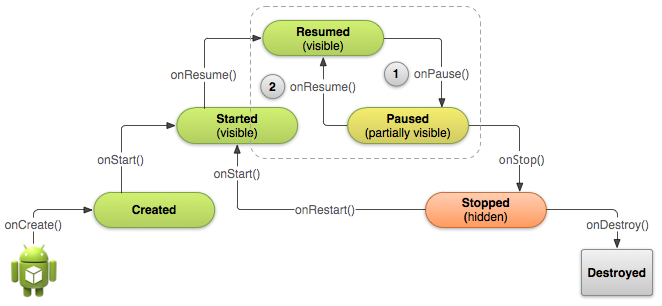
\includegraphics[scale=0.5]{basic-lifecycle-paused}

또 다른 케이스를 들어보자.
\begin{enumerate}
\item onCreate()에서 finish()를 호출하면 다른 생명주기 메서드를 거치지 않고 곧바로 onDestroy()를 실행한다.
\item onActivityResult()는 onResume()보다 먼저 실행된다.
이 순서가 필요할 때가 있다. onActivityResult()에서 가져온 결과를 업데이트하고
onResume()에서도 최신 데이터를 업데이트하려고 할 때, 순서를 유념해야 한다.
\end{enumerate}

Activity에는 onPostCreate()나 onPostResume() 같은 메서드도 있어서 앞에서 얘기한 생명주기 메서드 사이에 뭔가를 할 수도 있지만, 시스템에서 초기화를 위해서 사용하는 것으로 일반적으로 앱에서는 쓰지 않도록 가이드하고 있다.

\subsection{startActivity()와 startActivityForResult()}
Activity를 시작하는 방법은 startActivity()와 startActivityForResult() 메소드를 호출하는 것이다. 대부분 Activity에서 다른 Activity를 시작하고 특별한 경우에 다른 컴포넌트에서 Activity를 시작한다.\\

어떤 책에서는 호출하는 쪽을 부모 Activity라고 하고, 호출되는 쪽을 자식 Activity라고 하는데 혼동스런 표현이다. TabActivity와 같은 ActivityGroup이 부모 Activity이고, 탭 위치에 들어가는 하위 Activity가 자식 Activity이다. Activity에도 getParent() 메서드가 있는데 이것은 자신을 포함(embed)한 Activity를 가리키는 것이지 자기를 호출한 Activity를 가리키는 것이 아니다. 
Activity에 getCallingActivity()와 getCallingPackage() 메서드가 있어서 이 관계를 더 잘 나타내는 말인 듯하여, 이 책에서는 Caller(호출자)와 Callee(피호출자)로 정하고 부르도록 한다.\\

startActivity()는 Callee에 데이터를 전달하기만 하고 Caller에게 다시 데이터를 전달하는 어떤 액션도 하지 않는다.
startActivity() 메서드는 Context의 메서드이므로 Activity뿐만 아니라 Service, BroadcastReceiver, Application 어디서든 startActivity()를 실행할 수 있다.
startActivity()로 시작된 Callee에서는 getCallingActivity()와 getCallingPackage() 메서드는 null을 리턴한다.

startActivityForResult()는 Activity의 메서드다. Activity끼리만 데이터를 주고받을 수 있다고 이해하자. 
startActivityForResult() 메서드 관련해서 몇 가지 내용을 살펴보자.
\begin{itemize} 
\item Callee에서 getCallingActivity()와 getCallingPackage() 메서드는 Caller의 정보를 리턴한다. Caller에 따라 다른 처리가 필요한 경우 구분을 위해 이용할 수 있다. 
\item startActivityForResult(Intent intent, int requestCode) 메서드 시그너처에서  requestCode는 0 이상인 값을 넣으면 된다.
\item 두 Activity가 다른 태스크에 속해 있다면 onActivityResult()에서 결과를 다시 받을 수 없다.
\item 결과를 돌려주는 Callee에서는 finish() 메서드 전에 setResult() 메서드를 호출해야 setResult(int resultCode, Intent data) 메서드의 파라미터인 resultCode와 data가 Caller에 전달된다. 보통 이런 실수를 하지 않지만 기능을 추가하다 보면 위치를 잘못 잡을 때가 있다.
\item setResult() 메서드를 호출하지 않으면 기본으로 RESULT\_CANCELED(0) 값이 전달된다. 일반적으로 RESULT\_OK(-1) 값을 넣지만, 임의로 원하는 정수값을 전달해도 된다.
\item ActivityA에서 startActivityForResult() 메서드로 ActivityB를 호출하고 ActivityB에서는 자신을 닫고 또 다른 ActivityC를 호출하는 경우가 있다. 
이때 ActivityC에서 setResult()를 실행해서 전달한 것은 ActivityA에 전달될까? 가끔 이것을 가정하고 만들어진 것도 있는데 전혀 그렇지 않다. 
ActivityC가 닫히는 순간 ActivityA의 onActivityResult() 메서드가 불리지만, setResult() 메서드의 파라미터인 resultCode와 data는 ActivityA에 전달되지 않고 resultCode는 RESULT\_CANCELED면서 data == null이 될 뿐이다.  이런 경우에 값을 전달받기 위해서는, ActivityB에서 ActivityC를 시작하기 위해서 startActivity()를 실행하면서 Intent에 Intent.FLAG\_ACTIVITY\_FORWARD\_RESULT 플래그를 추가하는 것이다.
이 플래그는 startActivityForResult()에서 쓰려고 하면 ``android.util.AndroidRuntimeExce\-ption: FORWARD\_RESULT\_F\-LAG used while also requesting a result''  예외를 발생시킨다. 
다시 말하면, ActivityA에서 ActivityB를 시작할 때는 startActivityForResult() 메서드를 사용하고, ActivityB에서 ActivityC를 시작할 때는 startActivity() 메서드를 사용하면서 플래그를 사용해야 한다. 
이런 식으로 하면 2개가 아닌 여러 개를 거쳐도 맨 아래에서 startActivityForResult()를 실행한 Activity에 값을 다시 전달할 수 있다.
\end{itemize}

\subsection{Activity 전환}
Activity가 전환되면서 생명주기 메소드가 어떻게 불리는지 알아보자.\\

\underline{\bfseries Activity에서 다른 Activity를 시작할 때}\\
ActivityA에서 ActivityB를 시작할 때, ActivityA는 onPause()와 onStop()을 실행할 것이고
ActivityB는 onCreate()와 onResume()을 실행할 것이다.
그런데 ActivityA가 onStop()까지 실행되고 나서 ActivityB가 onCreate()부터 실행되는 것이 아니다.
순서는 다음과 같다.
\begin{enumerate}
\item ActivityA는 onPause() 메서드를 실행한다(백그라운드로 이동).
\item ActivityB는 onCreate(), onStart(), onResume() 메서드를 실행하고 포커스를 갖는다(포그라운드로 이동).
\item ActivityA는 onStop() 메서드를 실행한다(ActivityA는 not visible. ActivityB가 전체 화면을 덮는 경우). ActivityB가 반투명이거나 다이얼로그 테마 Activity인 경우에는 onStop()을 실행하지 않는다(아직 visible이기 때문).
\end{enumerate}

설명해보면 Caller는 일단 백그라운드로 가고, Callee가 포그라운드까지 온 다음에 Caller가 not visible 상태가 된다.
onStop()이 나중에 불리는 이유는 무엇일까? 
바로 Callee가 투명하거나 전체를 덮는 Activity가 아니라면 Caller의 onStop()을 호출하기 않기 때문에, 
Callee가 뜨고 난 이후에야 onStop()이 필요한지 알 수 있기 때문이다.\\

이 순서는 별게 아니지만 인지해야 하는 경우가 있다. 
ActivityA에서 변경된 값을 ActivityB에서 사용하고자 한다.
이때 ActivityA에서 매 이벤트마다 
SharedPreferences나 DB에 저장하지는 않고 ActivityA가 끝날 때만 저장하기로 했다.
이때 onStop() 메서드에서 저장하면 안되고 onPause() 메서드에서 저장해야만, ActivityB에서 이 값을 정상적으로 사용할 수 있다.\\

\underline{\bfseries 포그라운드 Activity가 닫힐 때}\\
앞과 반대 경우이다. 
ActivityA에서 ActivityB를 시작하고, 이번에는 ActivityB를 닫으면 ActivityA를 다시 보게 된다.
이때의 순서는 역순이다.
\begin{enumerate}
\item ActivityB는 onPause() 메서드를 실행한다(백그라운드로 이동).
\item ActivityA는 onRestart(), onStart(), onResume() 메서드를 실행한다(포그라운드로 이동).
\item ActivityB는 onStop(), onDestroy() 메서드를 실행한다(종료).
\end{enumerate}


\subsection{생명주기 메서드 사용 시 주의점}
\subsubsection{리소스 생성/제거}
onCreate()에서 리소스를 생성했다면 onDestroy()에서 제거하고, onResume()에서 생성했다면 onPause()에서 제거한다.
가장 많이 사용하는 예로는 onResume()에서 registerReceiver()를 실행하고, onPause()에서 unregisterReceiver()를 실행하는 것이다. 즉 포그라운드에 있을 때만 Broadcast 이벤트에 대해 처리하겠다는 것이다. 다른 예로 DB를 열고 닫는 것도 생각할 수 있다.
onCreate()에서 DB를 열었는데 onPause()에서 DB를 닫는다면 어떻게 될까?
다른 Acivity로 전환되었다가 다시 화면에 돌아올 때 onCreate()가 호출되지 않고 onResume()만 불리므로, 닫혀진 DB를 갖게 되고 쿼리를 실행할 수 없게 된다.

\subsubsection{super.onXxx() 호출 순서}
onCreate(), onResume()에서는 super.onCreate(), super.onResume()을 먼저 실행하고, 
onPause(), onDestroy()에서는 super.onPause(), super.onDestroy()를 나중에 실행한다.\\

\begin{lstlisting}[frame=single]
	protected void onCreate() {
    	super.onCreate();
    	...
	}

	protected void onResume() {
    	super.onResume();
    	...
	}

	protected void onPause() {
		...
		super.onPause();
	}

	protected void onDestroy() {
    	...
		super.onDestroy();
	}
\end{lstlisting}
생명주기를 시작할 때는 뭔가를 만들어내는 일이 많고, 끝날 때는 정리하는 일이 많다는 것을 생각하자.
구글에서 만든 소스나 샘플, 많은 책에서도 이런 규칙은 없고 이런 규칙에 맞게 작성하지도 않지만, 경험상 이 습관은 필요하다. \url{http://orhanobut.github.io/effective-android/}에서도 항목 37에 ``Constructive first, destructive last'' 내용이 있는 것을 볼 수 있다.\\

Activity의 onCreate()나 onResume(), onPause() 메서드에서는 실제로 하는 작업은 거의 없다.
onDestroy()에서는 하는 작업이 있긴 하다. 
startManagingCursor() 메서드에(허니콤에서 Deprecation되었지만) 등록되었던 Cursor를 닫고,
showDialog()를 사용해서 캐시된 Dialog를 제거한다.\\

일반적인 앱에서는 로그인/로그아웃 상태를 갖고 있거나 화면 로딩 속도를 체크하거나 하는 공통 로직이 있어서, 상위 클래스로서 BaseActivity를 사용하는 경우가 많다.
상위 클래스의 onResume() 메서드에서 객체 인스턴스를 하나 생성한다고 해보자. 
하위 클래스에서 onResume()에서 생성한 인스턴스를 가지고 로그를 찍을 수도 있고, 뭔가 추가적인 작업을 할 여지가 있다. 
그런데 super.onResume()을 먼저 호출하지 않고 나중에 호출하면 무슨 일이 생길까? 바로 개발 시에 자주 보는 NullPointerException을 만나게 된다.
onPause() 메서드에서는 super.onPause() 메서드를 먼저 호출하고서 다른 로직을 실행하면
이미 반납된 자원을 사용하는 경우가 생길 수 있다.\\

해당 샘플을 보자.
\begin{lstlisting}[frame=single]
public class BaseActivity extends Activity {

	protected MyLocationManager myLocationManager;

	@Override
	protected void onResume() {
		super.onResume();
		myLocationManager = new MyLocationManager();
		myLocationManager.requestUpdate();
	}

	@Override
	protected void onPause() {
		myLocationManager = null;
		super.onPause();
	}
}
\end{lstlisting}
여기서 myLocationManager 변수를 onResume()에서 생성하고 onPause()에서 null로 하였다. myLocationManager는 protected 변수로 하위 클래스에서도 사용한다.

\begin{lstlisting}[frame=single]
public class LocationActivity extends BaseActivity {

	private LocationRepository locationRepository;
	private Location lastLocation;

	@Override
	protected void onCreate(Bundle savedInstanceState) {
		super.onCreate(savedInstanceState);
		...
		locationRepository = new LocationRepository();
	}

	@Override
	protected void onResume() {
		lastLocation = locationRepository.getLastLocation();
		super.onResume();
	}

	@Override
	protected void onPause() {
		super.onPause();
		locationRepository.saveLocation(myLocationManager.getLastLocation()); // (1)
	}

}
\end{lstlisting}
하위 클래스에서는 onResume()에서 마지막 위치(lastLocation)을 가져오고 onPause()에서 마지막 위치를 저장한다. onPause() 메서드에서는 반례로서 super.onPause()를 먼저 호출하였다. 이때 super.onPause()에서 myLocationManager는 null로 만들었으므로 22라인(1)에서 NullPointerException이 발생한다. 21라인과 22라인 위치를 바꾸면 예외가 발생하지 않는다. 

\subsubsection{finish() 메서드 호출하고 바로 리턴}
onCreate() 메서드에서 유효성 여부를 체크하고 문제가 있을 때 토스트 메시지를 띄우고 finish()를 호출하고서 곧바로 리턴하지 않는 경우가 있다. finish() 메서드는 리턴 대용도 아니고 리턴을 포함한 것도 아니다. finish()는 Activity를 끝내라고 Message를 보내는 것일 뿐이다. finish()를 호출한 후에 그 아래 로직도 실행되면 당연히 유효성 문제가 있던 것을 진행했으므로 에러가 나거나 엉뚱한 결과를 보여줄 수 있다. finish() 호출 위치가 메서드의 끝일 때만 리턴이 필요 없는 것이지 메서드 중간이라면 리턴은 반드시 필요하다.

\subsubsection{on.Xxx() 메서드는 직접 호출하지 않음}
onCreate(), onResume(), onPause(), onDestroy() 메서드를 직접 호출하는 경우는 거의 볼 수 없지만, onBackPressed() 같은 메서드를 호출하는 경우는 가끔 보게 된다.
onBackPressed()는 기본 동작이 finish()를 호출하는 것이므로 일단 당장은 되지만, onBackPressed()는 요구 사항에 따라 변경될 여지가 있는 메서드이다.
사용 패턴을 알기 위해서 Back 키를 체크하는 코드가 들어갈 수도 있고, moveToTaskBack() 메서드처럼 태스크를 아예 백그라운드로 보내는 경우도 있다. 또는 Back 키를 막기 위해서 onBackPressed() 메서드에서 super.onBackPressed()를 쓰지 않고 비어있는 메서드로 오버라이드하기도 한다. 이때 onBackPressed()를 호출한 쪽은 동작에 문제가 생긴다. 
다른 코드에 영향을 쉽게 받는 코드는 가능하면 작성하지 않는 것이 좋다.\\

Activity와는 별개지만 SQLiteOpenHelper를 상속한 Database Helper를 만들 때 onUpgrade() 메서드에서 onCreate() 메서드를 호출하는 것은 여러 책에서도 흔히 보인다.
\begin{lstlisting}[frame=single]
@Override
public void onCreate(SQLiteDatabase db) {
    db.exexSQL("CREATE TABLE schedule ....");
    db.execSQL("INSERT INTO schedule VALUES ...");
    ...
    db.execSQL("CREATE TABLE member ...");
    ...
}

@Override
public void onUpgrade(SQLiteDatabase db, int oldVersion, int newVersion) {
   db.execSQL("DROP TABLE IF EXISTS schedule");
   db.execSQL("DROP TABLE IF EXISTS member");
   onCreate(db);
}
\end{lstlisting}
이것 역시 마찬가지다. 현재까지는 동작이 동일한 게 확실하다면, 별도 메서드를 만들어서 그 메서드를 호출하도록 하자.

\begin{lstlisting}[frame=single]
@Override
public void onCreate(SQLiteDatabase db) {
   createTables(db);
}

@Override
public void onUpgrade(SQLiteDatabase db, int oldVersion, int newVersion) {
   db.execSQL("DROP TABLE IF EXISTS schedule");
   db.execSQL("DROP TABLE IF EXISTS member");
   createTables(db);
}

private void createTables(SQLiteDatabase db) {
	db.execSQL("CREATE TABLE schedule ....");
    db.execSQL("INSERT INTO schedule VALUES ...");
    ...
    db.execSQL("CREATE TABLE member ...");
    ...
}
\end{lstlisting}

시스템이 알아서 호출하는 메서드는 함부로 엮어 주지 말고, 위처럼 별도 메서드를 만들도록 하자. 그럼으로써 한쪽의 메서드가 변경될 필요가 있어도 다른 곳까지 신경쓰지 않아도 된다.
``기능이 완전히 동일한데?''하고 반문하는 경우도 있다. 혼자서 개발한다면 문제가 되지 않는다. 하지만 여러 사람이 개발하는 동안에 자신이 바꾸는 코드가 어디까지 영향을 주는 지 매번 생각해야 한다면 피곤할 수 밖에 없다. 
코드를 읽은 것도 어려워진다. 
필자의 경우에는 Activity에 로그인하는 기능이 있다는데, 아무리 봐도 로그인하는 코드가 보이지 않아서 어려움을 겪은 적이 있다. 
원인은 코드 상에서 onActivityResult()를 직접 호출하고 그 안에서 로그인을 시도하는 것 때문이었다. onActivityResult()는 Callee에서 데이터를 받아서 처리하는 것이지 직접 호출하는 용도는 아니다.

\section{Configuration 변경}
% ActivityStack의 ensureActivityConfigurationLocked에서  Relauch할 것인지, 있던 것을 쓸 것인지 결정한다.
Configuration은 컴포넌트에서 어떤 리소스를 사용할 지를 결정하는 조건이고, 이 조건은 항목이 정해져 있다. 
%Configuration은 구성 또는 설정으로 번역된다. 환경 설정과 구분이 필요하고 안드로이드 개발자 사이트에도 한국어 번역이 구성으로 되어 있어, 여기서도 구성으로 용어를 사용하기로 한다.
%http://developer.android.com/intl/ko/guide/topics/manifest/activity-element.html
%http://developer.android.com/intl/ko/guide/topics/resources/runtime-changes.html
%http://developer.android.com/intl/ko/reference/android/content/res/Configuration.html
\pageref{flow}페이지에서 화면 회전 시 Activity의 생명주기 메서드는 onDestroy()까지 실행되고 다시 onCreate()부터 실행하는 것을 얘기했다. 
화면 방향(orientation)은 Configuration의 가장 대표적인 항목이고, 
android.content.res.Configuration에서 멤버 변수를 나열해보자. 
densityDpi,
fontScale,
hardKeyboardHidden,
keyboard,
keyboardHidden,
locale,
mcc,
mnc, 
navigation, 
navigationHidden,
orientation,
screeenHeightDp,
screenLayout, 
screenWidthDp,
smalllestScreenWidthDp,
touchScreen,
uiMode로 모두 17개가 있고, 
여기서 fontScale과 locale은 환경설정에서 정할 수 있는 사용자 옵션이고 나머지는 단말의 현재 상태이다.\\

\subsection{리소스 반영}
Configuration은 컴포넌트에서 사용하는 리소스를 결정하기 때문에,  Configuration이 변경되면 컴포넌트에서 사용하는 리소스도 변경된다. 예를 들어, 단말 환경설정에서 언어를 변경한다고 하자. 영어를 기본으로 한국어와 일본어를 지원하기 위해서 /res/values와 /res/values-ko과 /res/values-ja에 동일한 내용의 문자열을 번역해서 strings.xml을 각각 만든다. 단말의 처음 언어설정은 한국어여서 Activity 화면에 /res/values-ko/strings.xml의 문자열을 보여주고 있었는데, 언어설정을 일본어로 바꾸면 /res/values-ja/strings.xml의 문자열로 변경해서 화면에 보여줘야 하는데 어떤 방식으로 하는 것일까?
이를 위해 안드로이드에서 선택한 방법은 화면에서 하나씩 문자열을 찾아서 변경하지 않고 Activity를 재시작하고 변경된 리소스를 사용하는 것이다.
화면 회전도 마찬가지다. 화면 회전에 따라 /res/layout-port와 /res/layout-land 디렉터리의 레이아웃을 교체하려면 Activity를 재시작한다. 참고로 Activity 외에 다른 컴포넌트는 재시작하지 않는다.\\

Configuration 변경으로 인한 Activity 재시작은 하나의 인스턴스를 가지고 새로 초기화해서 재사용하는 것이 아니다. 기존 인스턴스는 onDestroy()까지 실행하고 새 인스턴스를 onCreate()부터 실행하는 것이다. 여기서 생길 수 있는 문제가 메모리 누수이다. Activity가 onDestroy()까지 불리었는데도 어느 곳에 Activity에 대한 참조가 남아있다면 이 Activity는 계속 GC 되지 않고 메모리를 차지하게 된다. 화면을 자꾸 회전할 때 OutOfMemoryError가 발생한다면 원인은 메모리 누수 때문이다. 빈번하게 발생하는 Activity의 메모리 누수 상황을 나열해보자.

\begin{itemize}
\item 떠있는 Activity에 특별한 작업을 하기 위해서 Activity 인스턴스를 Collection에 모아둔다. 최악의 상황으로 WeakReference를 사용한다고 해도 가능하면 피해야 한다. 기능 요구 사항이나 레거시 코드 문제로 사용한 적은 있지만 권장되지 않는 방식이다. Activity 목록은 시스템이 알아서 관리하는 영역이기도 하고, Activity가 종료할 때 Collection에서 제거해야 하는데 빠뜨리는 실수가 발생할 가능성도 많다.
\item Activity의 내부 클래스나 익명 클래스의 인스턴스가 Activity에 대한 참조를 갖고 있기 때문에, 외부에 리스너로 등록한 경우에 해제도 반드시 되어야만 한다. 메모리 누수의 많은 부분을 차지하고 있다. 내부 클래스에서 SomeActivity.this를 쓸 수 있는 상황, 즉 Activity 참조를 갖는 것을 없애기 위해 단순 내부 클래스는 정적 내부 클래스를 만드는 것이 권장된다.
이때 Activity의 변수나 메소드에 꼭 접근할 일이 있다면 정적 내부 클래스 생성자에 WeakReference로 Activity를 전달하기도 한다. 
그러면서 코드가 복잡해지는데 문제가 심각하다면 고려할 수 있는 방법이다. 
\item 싱글톤에 Context가 전달되어야 하는데 Activity 자신을 전달한 경우이다. 싱글톤에 Activity 참조가 남아서 문제를 일으킨다. 이에 대한 대응 패턴은 \ref{sec:singleton} 절 내용을 참고하자.
\item AsyncTask에서 작업이 오래 걸리는 경우에도 문제를 발생시킨다. Activity가 시작하면서 작업을 실행하기 위해서 onCreate()에서 AsyncTask를 시작한다고 하자. AsyncTask는 Activity에 대한 참조를 가지고 있기 때문에, 화면이 회전하고 onDestroy()가 불린다고 해서 AsyncTask가 끝나기 전까지는 GC 대상이 되지 않는다. 게다가 onCreate()에서 실행하기 때문에 회전할 때마다 AsyncTask는 매번 실행된다. Activity 자체나 AsyncTask 작업이 메모리를 많이 차지하고 AsyncTask가 시간이 오래 걸리는 조건에서, 화면까지 빈번하게 회전한다면 OutOfMemoryError 가능성이 높아진다. 이에 대해서 \ref{sec:asynctask} 절에서 대응 방법을 언급하였다.
\end{itemize}

언어별 문자열이 따로 없거나 가로/세로 모드 레이아웃이 별도로 없는 경우에도 일단 재시작한다. Configuration이 변경되면 무조건 재시작하는 것으로 이해하면 된다. 재시작해서 리소스를 가져올 때 결과적으로 동일한 리소스를 사용하는 것 뿐이다. 프레임워크에서 호출 스택은 아래와 같다.
%System Configuration 때문에 조금 혼동되기도 한다.

\lstset{basicstyle=\fontfamily{mono}\selectfont\footnotesize}
\begin{lstlisting}[frame=single]
ActivityManagerService.updateConfigurationLocked(Configuration values,
	ActivityRecord starting, boolean persistent, boolean initLocale)
	ActivityThread.applyConfigurationToResources(Configuration config) (through binder IPC)
		ResourcesManager.applyConfigurationToResourcesLocked(Configuration config, 	CompatibilityInfo compat)
			Resources.updateConfiguration(Configuration config, DisplayMetrics metrics, CompatibilityInfo compat)
				AssetManager.setConfiguration(int mcc, int mnc, String locale,
            		int orientation, int touchscreen, int density, int keyboard,
            		int keyboardHidden, int navigation, int screenWidth, int screenHeight,
            		int smallestScreenWidthDp, int screenWidthDp, int screenHeightDp,
            		int screenLayout, int uiMode, int majorVersion) (native method)
\end{lstlisting}
\lstset{basicstyle=\ttfamily\small}
Configuration이 변경되면 system\_server에서 동작하는 ActivityManagerService에서 앱 프로세스의 메인 클래스인 ActivityThread에 새로운 Configuration을 반영하도록 전달하고, 결과적으로 하는 일은 AssetManager의 네이티브 메서드인 setConfiguration()을 실행하는 것이다. 네이티브에서는 리소스 테이블을 유지하고 있는데 현재 Configuration을 전달해놓고, 리소스를 가져올 때마다 현재 Configuration에 맞는 리소스를 선택해서 가져온다.
이제 리소스를 가져오는 한 예로서 getText() 메서드의 호출 스택을 살펴보자.
\begin{lstlisting}[frame=single]
Resources.getText(int id)
	AssetManager.getResourceText(int ident)
		AssetManager loadResourceValue(int ident, short density,
			TypedValue outValue, boolean resolve) (native method)
\end{lstlisting}
결론적으로 AssetManager에 현재 Configuration을 전달하고, AssetManager를 거쳐서 Configuration에 맞는 리소스를 매번 선택해서 가져오는 것이다. 리소스 선택 로직은 내부적으로 최적화되어 있다. 안드로이드 개발자 사이트에서 `Providing Resources' 문서\footnote{http://developer.android.com/intl/ko/guide/topics/resources/providing-resources.html}에서 `Android가 가장 잘 일치하는 리소스를 찾는 방법'을 참고하자.\\
% 화면 회전은 WindowManagerService에서... 또는 setRequestOrientation도 가능...      

%http://developer.android.com/intl/ko/guide/topics/resources/providing-resources.html 구성한정자

\subsection{Configuration qualifier}
이제 리소스 디렉터리명을 구성하는 Configuration qualifier\footnote{구성 한정자 또는 리소스 식별자로 번역된다. 개발자 가이드에서는 구성 한정자로 쓰고 있다.}를 살펴보자. 개발자 가이드에 있는 우선순위대로 나열하였다.\\

\begin{longtable}{|c|c|c|}\hline
Configuration qualifier & 샘플 & Configuration 필드 \\ \hline
MCC 및 MNC	& mcc310, mcc310-mnc004  & mcc, mnc \\ \hline
언어 및 지역 & en, fr, en-rUS, fr-rFR & locale \\ \cline{1-2}
레이아웃 방향	& ldrtl, ldltr & \\ \hline
smallestWidth & sw320dp, sw600dp, sw720dp & smallestScreenWidthDp \\ \hline
이용 가능한 너비 & w720dp, w1024dp & screenWidthDp \\ \hline
이용 가능한 높이 & h720dp, h1024dp & screenHeightDp \\ \hline
화면 크기 & small, normal, large, xlarge & screenLayout \\  \cline{1-2}
화면 비율 & long, notlong & \\ \hline
화면 방향 & port, land & orientation \\ \hline
UI 모드	& car, desk, television, appliance, watch & uiMode\\ \cline{1-2}
야간 모드	 & night, notnight &  \\ \hline
화면 픽셀 밀도(dpi) &	\makecell{ldpi, mdpi, hdpi, xhdpi, xxhdpi, \\ xxxhdpi, nodpi, tvdpi} & densityDpi\\ \hline
터치 스크린 유형 &	notouch, finger	& touchscreen \\ \hline
키보드 가용성 & keysexposed, keyshidden, keyssoft	& \makecell{hardKeyboardHidden, \\ keyboardHidden} \\ \hline
기본 텍스트 입력 메서드	& nokeys, qwerty, 12key & keyboard \\ \hline
탐색 키 가용성 & navexposed, navhidden	 & navigationHidden \\ \hline
기본 비터치 탐색 메서드 & nonav, dpad, trackball & navigation \\ \hline
플랫폼 버전(API 레벨) & v4, v7, v11 & \\ \hline
\end{longtable}

Configuration qualifier에 대한 상세 내용은 `Providing Resources' 문서에서 표 2를 참고하고 여기서는 특기할 내용만 살펴보자.
\begin{itemize}
\item 플랫폼 버전도 리소스 선택에 영향을 미치지만  Configuration 필드에는 없다. 플랫폼 버전은 hidden 필드인 Build.VERSION.RESOURCES\_SDK\_INT에 상수로 되어 있다. 
\item Configuration 가운데서 fontScale은 Configuration qualifier와 관련된 것이 없다. 즉, fontScale은 리소스 선택 로직에는 영향을 주지 않고 Activity를 재시작하면서 화면에서 sp 단위로 된 문자열의 크기를 변경할 뿐이다.
\item 언어 설정을 아랍어, 히브리어 또는 페르시아어로 변경하면 RTL(right-to-left)로 레이아웃 방향이 변경된다(AndroidManifest.xml에서 supportsRtl=``true''이고 targetSdkVersion이 17이상). 예를 들어, horizontal LinearLayout에 ImageView와 TextView를 배치한다면 일반적인 LTR(left-to-right) 배치가 아닌 미러링 배치를 보게 된다. 즉 오른쪽에 ImageView가 있고 그 왼쪽에 TextView가 보인다. 환경설정의 개발자 옵션에서 `RTL 레이아웃 강제 변경'을 체크하면 한국어에서도 레이아웃 변화를 테스트할 수 있다. 
\end{itemize}
% mcclist.com에 mcc/mnc 리스트가 보인다. 통신사마다 다르게 리소스를 구성하고 싶을 때 사용한다.

\subsection{데이터 복구}
Configuration 변경으로 Activity가 재시작되어도 사용자 경험상 기존에 보던 화면을 가능하면 유지하는 게 좋다. 예를 들어, ViewPager에서 플링(fling)을 통해 특정 페이지로 이동했을 때 Configuration 변경에도 동일한 페이지를 보여주려고 한다. 이때 상태를 임시 저장하고 복구하는 메서드인 onSaveInstanceState()와 onRestoreInstanceState()를 사용하면 된다. onRestoreInstanceState() 메서드에 전달되는 Bundle savedInstanceState 파라미터는 onCreate() 메서드에도 전달되지만, 대칭을 위해서 onRestoreInstanceState() 메서드에서 복구하는 로직을 많이 사용한다.
% onSaveInstance 메소드는 onPause 이전에 호출된다. 
% onRestoreInstanceState는 onCreate 메소드이후, onResume 메소드 이전에 실행된다.
% 하니콤 이전과 이후에 대해서 확인 필요하다.
onSaveInstanceState(), onRestoreInstanceState() 메소드는 Configuration 변경으로 재시작할 때 뿐만 아니라, 메모리 문제로 시스템이 Activity를 kill하는 경우(주로 백그라운드에 있을 때 우선순위에 밀려서 발생)에도 호출된다\\

onSaveInstanceState()는 생명주기 메서드처럼 항상 호출되는 것이 아니다.
각 생명주기마다 로그를 남겨서 실행 여부를 체크해보면, onSaveInstanceState()는 호출되지 않는 것을 알 수 있다. 
Configuration 변경되는 조건에서(가장 손쉽게 화면을 회전해보면) onSaveInstanceState()가 호출되고 Activity는 onCreate()부터 재시작한다.\\

이제 한 가지 의문을 가져보자.
앱에 여러 Activity가 있어서, ActivityA$\rightarrow$ActivityB$\rightarrow$ActivityC 순으로 태스크에 쌓였다. 이때 화면을 회전하면 세 개의 Activity에서 모두 onSaveInstanceState()가 호출될 것인가? 그렇지 않다.
ActivityA$\rightarrow$ActivityB$\rightarrow$ActivityC 순으로 하면 앞의 Activity는 onStop()이 호출되는데, onStop 이전에 onSaveInstanceState()가 호출된다.
즉 ActivityA, ActivityB는 onSaveInstanceState()가 호출된 상태이다.\\

이 상태에서 ActivityC를 회전하면 ActivityC에서는 기대하는 대로 onSaveInstanceState() 실행 이후에 재시작한다.
이제 Back 키로 ActivityC를 종료하면 onSaveInstanceState()가 이미 호출된 ActivityB는 이제서야 재시작한다.\\

ActityC를 회전했다가 다시 원래대로 돌린 다음에 Back 키로 돌아가면 어떨까? 즉 ActityB로 보면 방향이 바뀌지 않은 것이다.
이때는 ActivityB를 재시작하지 않는다. 즉 화면이 덮이는 상황에서는 onSaveInstanceState()를 해놓지만, 다시 돌아왔을 때 Configuration이 바뀌지 않는다면 화면을 그대로 보여줄 뿐 복구할 내용이 없는 것이다.\\

ActivityC에서 Home 키를 누르면 어떻게 될까? 이때도 ActivityC는 onSaveInstanceState()를 호출해 놓는다.
이후에 다시 포그라운드로 돌아올 때, 만일 화면 방향 등의 Configuration이 변경되었다면 ActivityC를 재시작한다. Power 키로 화면을 OFF하는 경우도 동일하다. onStop() 메서드까지 실행되는데 직전에 onSaveInstanceState()를 호출한다. 그래서 화면 방향이 바뀌고서 화면이 ON되는 순간에도 데이터를 복구할 수 있다.\\

ActivityA$\rightarrow$ActivityB$\rightarrow$DialogActivity(다이얼로그 테마)의 경우는 어떨까?
DialogActivity가 뜨면 아직 배경으로 보이는 ActivityB의 onSaveInstanceState()는 호출된다.
이때 화면을 회전하면 DialogActivity에서 onSaveInstanceState() 호출 후 재시작하고 그 이후에 ActivityB를 재시작한다.\\

\subsection{android:configChanges 속성}
앞에서도 얘기했듯이 Configuration 변경 가운데서 가장 빈번하게 발생하는 것은 화면 회전이다. 화면 회전 시에 매번 재시작해서 Activity 초기화 때문에 느려지는 것이나 상태 저장/복구에 부담을 느낄 때, 재시작을 방지하기 위해서 AndroidManifest.xml의 Activity 선언에 지정하는 속성은 2가지가 있다.
\begin{itemize}
\item android:screenOrientation 속성을 ``portrait''나 ``landscape''로 고정해서 회전해도 화면은 그대로이고 재시작이 일어나지 않게 한다. 화면이 상대적으로 작은 2.X 버전에서는 화면 방향을 고정하는 경우가 많았는데, 태블릿을 지원하는 3.X 버전 이후에는 많이 쓰이지 않는다. 게임 앱과 같이 용도가 확실한 것에도 화면 방향을 고정하는데, 요구 사항에 맞다면 쓸 수 있는 옵션이다. 이때 화면 회전 시에도 Configuration은 변경되지 않는다.
\item android:configChanges 속성에 ``orientation''을 지정해서 화면 회전 시에는 재시작하지 않고 Activity의 onConfigurationChanged() 메서드에서 회전 시에 할 작업을 지정한다.
\end{itemize}

첫 번째 내용은 굳이 더 얘기할 게 없고 두 번째 내용에 주목하자.
%http://developer.android.com/intl/ko/guide/topics/manifest/activity-element.html
%http://developer.android.com/intl/ko/reference/android/R.attr.html#configChanges
android:configChanges 속성에 들어가는 내용은 아래 항목과 그 비트 OR 값($|$)이다.\\
mcc, mnc, locale,
touchscreen, keyboard, keyboardHidden, 
navigation, orientation, screenLayout, uiMode, screenSize,
smallestScreenSize, layoutDirection, fontScale\\

이 항목은 안드로이드 개발자 사이트에서도 개수가 잘 맞지 않는다. \url{http://developer.android.com/intl/ko/reference/android/R.attr.html\#configChanges}에는 14개가 모두 나오지만 http://developer.android.com/intl/ko/guide/topics/manifest/activity-element.html에는 현 시점에서(2016년 1월) layoutDirection이 나오지 않기도 한다.\\

Configuration 변수명과 차이가 있는 것도 혼동스럽다. 이 항목들은 비트 OR 연산을 위해서 숫자 상수와 매핑되는데 android.content.pm.ActivityInfo에서 CONFIG\_로 시작하는 상수가 그 값이다.
ActivityInfo에는 CONFIG\_DENSITY도 있지만 이 상수는 사용되지 않는다.
이름이 동일한 것을 제외하고 나머지는 어떻게 매핑되는지 표로 살펴보자. 표의 내용은 Configuration에서 비트 OR 연산을 하는 updateFrom() 메서드를 참고하였다.\\

\begin{tabular}{|c|c|}\hline
Configuration & android:configChanges \\ \hline
densityDpi & 없음 \\ \hline
screeenHeightDp, screenWidthDp & screenSize \\ \hline
hardKeyboardHidden, navigationHidden  & keyboardHidden  \\ \hline
smallestScreenWidthDp & smallestScreenSize \\ \hline
\end{tabular}\\

여기서 특이한 것은 navigationHidden이 keyboardHidden에 매핑된다는 것이다. navigation에 매핑되지 않을까 생각했는데, navigation은 내비게이션 타입(trackball/dpad)이 바뀐 것을 의미한다.\\

android:configChanges에 넣는 항목에 대해서는 Configuration 변경에 대해서 처리할 내용이 없거나, onConfigurationChanged()를 오버라이드해서 직접 처리하겠다는 의미이다. onConfigurationChanged()가 불린 이후에는 화면을 다시 그린다. onConfigurationChanged()를 따로 오버라이드하지 않아도, 화면이 회전할 때 세로 모드에서 View의 layout\_width가 MATCH\_PARENT였다면 가로 모드로 바뀌었을 때 가로 모드 너비에 맞게 꽉 채워서 다시 그려주는 것을 보면 알 수 있다.\\

%그럼 직접 처리한다는 건 또 무슨 의미일까?
android:configChanges에 항목을 넣어서 활용하는 경우를 예를 들어보자. 
onConfigurationChanged()에는 변경된 Configuration에 대한 리소스가 사용 가능한 것을 기억하자. 
\begin{itemize}
\item 가장 흔한 경우로 화면 회전에 대응하는 orientation이 있다. -port, -land로 별도 레이아웃을 사용하지 않을 때 많이 쓰인다. 앞에서 얘기했듯이 onConfigurationChanged()가 실행된 이후에 다시 그려지면서 View의 layout\_width나 layout\_height가 바뀐 것은 아니지만, 그려진 너비와 높이는 measure된 결과에 따라서 달라진다.
경우에 따라 가로/세로 모드에서 layout\_width나 layout\_height만 변경해서 적용하려고 할 때도 있다. 
예를 들어, Master-Detail 화면에서 세로 모드에서는 Master 너비를 크게 쓸 수 없었지만 가로 모드에서는 좀 더 여유있게 쓸 수 있다. 전체 레이아웃이 바뀌지 않는 정도에서는 -port, -land로 별도 레이아웃을 만들 필요는 없다.
바로 /res/valuse-port와 /res/values-port에 dimens.xml에 각각 동일한 name로 값을 넣고 레이아웃에서 name을 참조하면 된다.
\begin{lstlisting}[frame=single, caption=/res/values-port/dimens.xml]
<?xml version="1.0" encoding="utf-8"?>
<resources>
	<dimen name="left_width">50dp</dimen>
</resources>
\end{lstlisting}

\begin{lstlisting}[frame=single, caption=/res/values-land/dimens.xml]
<?xml version="1.0" encoding="utf-8"?>
<resources>
	<dimen name="left_width">70dp</dimen>
</resources>
\end{lstlisting}

\begin{lstlisting}[frame=single, caption=/res/layout/view\_list.xml 일부분]
	<LinearLayout
		android:layout_width="match_parent"
		android:layout_height="150dp"
		android:orientation="horizontal">
		<View
			android:id="@+id/left"
			android:layout_width="@dimen/left_width"
			android:layout_height="match_parent"
			android:background="#00ff00" />
		<View android:layout_width="match_parent"
			android:layout_height="match_parent"
			android:background="#0000ff" />
	</LinearLayout>		
\end{lstlisting}
android:configChanges 속성을 쓰지 않는다면 화면을 회전할 때마다 그에 맞는 dimens.xml 파일을 참조해서 화면을 보여줄 것이다. 
android:configChanges 속성을 쓸 수도 있다. 이때는 onConfigurationChanged() 메서드를 오버라이드해야 한다.

\begin{lstlisting}[frame=single]
	private View left;

	@Override
	protected void onCreate(Bundle savedInstanceState) {
		super.onCreate(savedInstanceState);
		setContentView(R.layout.view_list);
		left = findViewById(R.id.left);
	}

	@Override
	public void onConfigurationChanged(Configuration newConfig) {
		super.onConfigurationChanged(newConfig);
		ViewGroup.LayoutParams lp = left.getLayoutParams();
		lp.width = getResources().getDimensionPixelSize(R.dimen.left_width);
		left.setLayoutParams(lp);
	}
\end{lstlisting}
onConfigurationChanged()에서 getResource().getXxx() 메서드는 변경된 Configuration에 대응되는 값을 가져오므로, 이 코드는 화면 회전에 따라 그에 맞는 dimens.xml의 값을 쓰겠다는 의미이다.\\

조금 혼동이 올 수도 있겠다. 어차피 다시 그릴텐데 리소스도 새로운 Configuration에 맞는 리소스를 선택해서 그리는 건 아닐까? 
즉 onConfigurationChanged()를 오버라이드하지 않아도 될 것 같다.
이것은 View의 생성자에서 해당 Configuration의 리소스를 대입하는 일반적인 구조 때문이다. 정확하게 얘기하면 android:layout\_width나 android:layout\_height는 View의 속성이라기보다 상위 ViewGroup의 속성으로, LayoutInflator의 inflate()에서 View 생성자에서 다른 속성은 모두 처리하고 나서, ViewGroup의 generateLayoutParams()를 실행해서 android:layout\_width나 android:layout\_height를 처리한다.
즉, /res/layout/view\_list.xml에서 android 네임스페이스에 있는 값들은 LayoutInflator의 inflate() 실행 순간에 이미 대입되고, Configuration이 변경된다고 해서 다시 대입되지 않는다. 
	
\item textSize로 sp를 쓰지 않는다면 fontScale도 가능하다. UI가 단순한 경우에는 권장사항대로 sp를 써도 되지만, UI가 복잡한 경우 디자인적인 문제로 textSize를 dp로 제한하는 경우가 많다.

\item 다국어 대응을 하지 않는다면 locale을 넣을 수도 있다. 또는 화면의 일부만 다국어 대응을 할 수도 있다. 타이틀만 변경해도 된다면 onConfigurationChanged() 메서드에서 titleText.setText(R.string.title)와 같이 쓰면 해당 언어로 문자열이 쓰여진다.
\end{itemize}

비트 OR 값에 대한 얘기도 필요하다. android:configChanges에 들어간 비트 OR 값은 그 중에 하나만 해당하면 되는 게 아니다. 그 비트 OR 값에 모두 포함되어야 Activity가 재시작하지 않고 onConfigurationChanged() 메서드에서 처리한다. 여러 조건이 한꺼번에 변경되는 경우가 있다. 예를 들어, 환경설정에서 언어를 바꾸고 화면을 회전하고서 Activity가 포그라운드로 돌아오면 locale과 orientation이 한꺼번에 바뀐다. 이때 android:configChanges에 orientation만 있고 locale이 포함되지 않는다면 Activity는 재시작한다. locale도 바뀌었는데 이에 대해 처리하는 방법이 없는 것으로 간주하는 것이다.\\

이 때문에 번거로운 게 있는데 꼭 같이 붙어다니는 항목들이 있다.
android:configChanges에 가장 보편적으로 들어가는 게 orientation인데, 허니콤 API 레벨 13 이상에서는 화면을 회전할 때 화면 크기도 같이 변경된다(targetSdkVersion이 그 이하이면 호환 모드로 동작).
앱을 업데이트하면서 targetSdkVersion을 올렸는데 화면 회전에 대해 기존처럼 동작하지 않는다면 이 때문이다. 
따라서 화면 회전을 정상적으로 처리하고자 할 때 screenSize도 함께 해서 ``orientation|screenSize''를 쓰면 된다.\\

그리고 화면 회전과 관련해서 keyboardHidden도 포함해서 ``keyboardHidden|orientation|screenSize''로 쓰는 경우가 많다.
왜 화면 회전에 관련 속성이 아닌 듯한 keyboardHidden(하드웨어 키보드가 숨겨졌는지 여부)이 따라붙는 것일까?ㅊ
근래에는 큰 화면이 많아서 별로 없지만, 초기에는 하드웨어 키보드가 있는 모델(2009년에 모토쿼티, 2010년에는 옵티머스 Q)이 있었다.
키보드가 겹쳐있다가 슬라이딩되면서 하드웨어 키보드가 나오는데, 세로 모드로 있다가 키보드를 나오는 순간에 단말을 돌린 것은 아니지만 가로 모드로 전환되었다. 이때 keyboardHidden 속성이 변경되면서 방향도 바뀌기 때문에 keyboardHidden과 orientation을 함께 쓰게 되었다.\\

Activity에는 setRequestedOrientation(int requestedOrientation) 메서드가 있다. 방향 센서를 통해서 화면을 회전하는 것이 아니라, 필요에 따라 특정 방향으로 화면을 보여줄 수 있는 메서드이다. 이 메서드를 호출하면 기본적으로 Activity는 재시작하는데, 이때도 android:configChanges에 orientation 항목이 있다면 재시작하지 않고 onConfigurationChanged() 메서드가 불린다.\\

android:configChanges에 값을 넣을 때는 `최대'보다는 `최소'를 원칙으로 하는 게 좋다. 14개를 다 넣는다고 Activity가 절대 재시작하지 않는 것도 아니다. 백그라운드로 이동했다가 kill되는 경우도 있어서 완벽한 대응이 되지 않는다. mcc와 mnc와 같이 유심이 새로 발견된 경우처럼 굳이 대응이 필요하지 않은 경우도 있다. 유심이 바뀐 경우 단말 재부팅하기도 바쁜데, 앱에서 Activity가 재시작하고 값을 복구하는지 신경쓸 사용자는 없을 것이다.\\

\begin{comment}
 \url{http://www.androiddesignpatterns.com/2013/04/retaining-objects-across-config-changes.html}에 따르면, android:configChanges 는 믿고쓰는 속성이 아니다. 
     
 android:configChages=``orientation''(예를 들어) 옵션을 쓰지 말라고 하고 있다.
단말 회전에 불필요하게 Activity를 재시작하는 비용 때문에 쓰는 경우가 있지만,
언어 설정 변경, 폰트 사이즈 변경 시에는 대응이 되지 않는다.
예를 들어 ViewPager에서 플링(fling)을 통해 특정 페이지로 이동했을 때, 화면 회전에도 페이지가 유지되지만 환경 설정에서 언어나 폰트 사이즈가 변경되면 다시 Activity가 생성되면서 ViewPager는 첫 번째 페이지가 나타나게 되다.
태스크가 백그라운드로 갔다가 다른 우선순위에 밀려서 kill되었을 때도 마찬가지다. 이때도 페이지가 유지되지 않는다.\\
\end{comment}

android:configChanges에 값을 넣어도 onSaveInstanceState()는 여전히 불린다. ``orientation|screenSize''로 설정한 경우를 보자.
ActivityA$\rightarrow$ActivityB$\rightarrow$ActivityC로 Activity를 전환하고, 화면을 회전하면 그때 재성성하지 않고 onConfigurationChanged() 메서드가 불리는 것이 다르다.
ActivityA$\rightarrow$ActivityB$\rightarrow$DialogActivity(다이얼로그 테마)에서는 화면을 회전하면 DialogActivity 먼저 onConfigurationChanged()가 불리고 ActivityB는 그 다음에 불린다.\\

결론적으로 빈번한 화면 회전에 대응하는 목적으로 android:configChanges를 사용하는 것은 나쁜 선택은 아니다.
다만, 이때 중요한 정보에 대해서는 onSaveInstanceState()와  onRestoreInstanceState()도 함께 사용하는 게 좋다.\\

\subsection{Configuration 확인}
마지막으로 Configuration을 확인하는 방법과 Configuration이 변경되는 타이밍에 대해서 더 알아보자.\\
 
Configuration 내용을 보기 위해서는 Context 인스턴스에서 getResources().getConfigura\-tion()으로 가져와서 Configuration의 toString() 메서드로 출력하면 된다. 
\begin{lstlisting}[frame=single]
{1.0 450mcc5mnc ko_KR ldltr sw360dp w360dp h567dp 480dpi nrml port finger -keyb/v/h -nav/h s.28}
{1.0 450mcc5mnc ko_KR ldltr sw360dp w598dp h335dp 480dpi nrml land finger -keyb/v/h -nav/h s.29}
...
{1.15 450mcc5mnc ko_KR ldltr sw360dp w360dp h567dp 480dpi nrml port finger -keyb/v/h -nav/h s.39}
{1.15 450mcc5mnc ko_KR ldltr sw360dp w598dp h335dp 480dpi nrml land finger -keyb/v/h -nav/h s.40}
\end{lstlisting}
값이 14개가 나오는데 실제 단말에서는 커스텀 데이터가 더 나오기도 한다. 1, 2라인은 화면을 회전한 것이고 4, 5라인은 설정에서 글꼴 크기를 키우고서 화면을 회전한 것이다.
\begin{itemize}
\item 첫 번째는 fontScale 값이다. `보통'인 경우 1.0이고(1, 2라인) `크게'인 경우 1.15가 나왔다(4, 5라인). 표준 비율은 있지만 단말마다 비율이 차이가 있어 실제 의미가 없다. `보통'에서는 값이 1.0인 것은 변함없을 것 같은데 갤럭시 노트4에서는 값이 1.09로 나오기도 했다.
\item 두 번째는 mcc, mnc 값이다. \url{http://mcclist.com}에 따르면 450은 한국의 국가 코드이고 5는 SK Telecom의 통신사 코드이다.
\item 세 번째는 locale 값이다.
\item 네 번째 ldltr은 screenLayout 값이다.
\item 다섯 번째 sw360dp는 smallestScreeWidthDp 값이다. 화면을 회전해도 이 값은 변하지 않는다.
\item 여섯 번째와 일곱 번째는 screenWidthDp와 screenHeightDp 값이다. 화면 회전 시에 width와 height가 서로 바뀌기만 할 것 같은데, 상단의 status bar 영역과 함께 Nexus 시리즈에 주로 보이는 Home 키를 포함한 소프트 키 영역 때문에 차이가 생긴다.
\item 여덟 번째는 densityDpi 값이다.
\item 아홉 번째 nrml은 screenLayout 값이다.
\item 열 번째는 orientation 값이다.
\item 열한 번째 finger는 touchScreen 값이다.
\item 열두 번째 -keyb/v/h는 keyboard, keyboardHidden, hardKeyboardHidden 값이다. v나 h는 visible/hidden의 의미다. -keyb는 키가 없다는 의미다(마이너스로 생각하면 된다).
\item 열세 번째 -nav/h는 navigation과 navigationHidden 값이다. 마이너스가 있으므로 navigation 타입이 없다는 것이다. 
\item 열네 번째 seq는 변경 횟수이다. Configuration이 바뀔 때마다 seq가 커진다. seq는 한 앱에 대한 것이 아니라 단말 전체적으로 쓰이는 전역적인 값이다.\footnote{seq는 ActivityManagerService의 updateConfigurationLocked() 메서드에서 변경한다.}
\end{itemize}

이제 Configuration이 변경되는 시점에 동작에 대해서 얘기해보자. Configuration이 바뀔 때는 Application의 onConfigurationChanged() 메서드가 먼저 불리고, 포그라운드에 있는 Activity는 AndroidManifest.xml 설정에 따라 재시작하거나 onConfigurationChanged() 메서드가 불린다.
화면 방향 관련해서 Configuration이 바뀌는 것은 포그라운드에 있는 Activity가 기준이다. 만일 화면 방향 고정인 Activity가 포그라운드에 있다면 아무리 화면을 회전해도 Application의 onConfigurationChanged()는 불리지 않는다. ActivityA가 화면 방향 가로 고정이고 ActivityB가 따로 방향을 고정하지 않았다면 어떤 현상이 발생할까? ActivityA의 Configuration orientaton은 land로 고정된다. 이때 Configuration seq가 N이라고 하면, ActivityA에서는 아무리 화면을 회전해도 seq가 바뀌지 않는다. ActivityB로 전환하면 어떤 현상이 발생할까? 만일 세로 방향이었다면 ActivityB가 세로 방향으로 보여야 하기 때문에 orientation이 port로 바뀌면서 seq는 N+1이 된다. 만일 가로 방향이었다면 seq는 그대로이다. 이제 ActivityB를 회전하면 계속해서 seq가 늘어나면서 land$\leftrightarrow$port가 서로 바뀐다. 이제 ActivityB를 종료하고 ActivityA로 돌아오면 어떻게 될까? 이 시점에 orientaton이 land라면 seq가 더해지지 않는다. 그런데 orientaton이 port라면 ActivityA에 맞는 Configuration으로 변경되면서 orientaton이 land가 되고 seq는 더해진다. seq는 변경될 때마다 Application의 onConfigurationChanged() 메서드가 불린다.\\

Configuration은 한순간에 1개의 값만 존재한다. 예를 들어, ActivityA 위에 다이얼로그 테마 ActivityB가 있다고 하자. 다이얼로그 테마 Activity에 android:screenOrientation을 지정하지 않으면(즉 unspecified라면) 배경에 있는 Activity의 방향을 따르므로 문제가 없는데, 이제 ActivityA의 android:screenOrientation=``land'이고 ActivityB의 android:screenOrientation=``port''로 다른 방향으로 해보자. 
ActivityA만 있을 때는 세로 고정이었는데, 가로 화면인 ActivityB를 시작하면 배경에 있는 ActivityA까지 가로로 바뀌어 버린다. 여기서 재미있는 현상이 발생한다. android:configChanges에 방향 회전에 대응되어 있다면 ActivityA의 onConfigurationChanged() 메서드가 불리고 그렇지 않다면 ActivityA는 재시작한다.  필자의 경우도 android:screenOrientation이 land나 port로 지정되면 방향 전환에 대해서 android:configChanges는 필요없다고 생각했는데 이런 특이한 케이스도 있다는 것을 생각하자.\\

% bg가 no option이고 fg가 landscape을 때 한번 landscape로 또 고정
% bg가 landscape이고 fg가 sensor을 때 매번 회전

앱의 Activity가 모두 종료되었을 때는 어떨까? 프로세스가 바로 종료되지 않고 Empty Process로 한동안 남아있는데, 이때도 포그라운드에 있는 다른 앱의 Activity가 방향 회전할 때마다 Application의 onConfigurationChanged() 메서드는 불린다. 
다른 앱의 Activity가 역시 방향 고정이라면 Application의 onConfigurationChanged() 메서드는 불리지 않는다. 보통 런처 앱은 방향 고정인 경우가 많아서 홈 화면에서 아무리 화면을 회전해도 다른 앱의 Configuration에 영향을 주지 않는다. 
Activity가 스택에 남아있는 채로 Home 키를 통해 백그라운드로 이동해도 마찬가지다. 포그라운드에 있는 Activity가 아닌 것은 변경된 Configuration을 받지 않으므로, 다른 앱에서 바뀐 Configuration은 Activity에는 전달되지 않고 Application에만 전달된다.\\

환경 설정에서 언어나 글꼴 크기를 변경할 때도 실행중인 모든 앱 프로세스에서 Application의 onConfigurationChanged()에 변경된 Configuration이 전달된다.\\




